\subsection{Techniques for pure shift optimisations}
\label{subsec:pureshift__optim_techniques}

Throughout this chapter (and more generally this thesis), various algorithms are used for \textit{optimisation}: that is, to find the parameters $\symbf{x} \in \mathbb{R}^n$ which minimise a \textit{cost function} $f : \mathbb{R}^n \to \mathbb{R}$.
These algorithms can loosely be categorised as either \textit{derivative-based} or \textit{derivative-free}: the former use extra information in the form of $\nabla f\/$ to help locate the optimum, whereas the latter do not, using only the value of $f(\symbf{x})$.
While derivative-based algorithms typically converge to an optimum more quickly, they are unsuitable for problems where the cost function $f\/$ is noisy.
In this section, the Nelder--Mead (NM) simplex algorithm\autocite{Nelder1965TCJ} was used: it is a very popular derivative-free method, and although mathematical convergence is not guaranteed\autocite{McKinnon1998SIAMJO}, in practice such cases are rather unlikely to arise.
In this section, the implementation of the NM algorithm in the Python \texttt{scipy} package was simply used as-is.

The cost function measuring the performance of a pure shift experiment can be measured in one of two ways: either \textit{theoretically}, in that the pure shift experiment is simulated using the density operator formalism, or \textit{experimentally}, in that the experiment is run on a spectrometer.
Unfortunately, the simulation of PSYCHE-type PSEs, where a shaped pulse is applied together with a gradient, requires a large amount of time.
The pulse itself already has $m \sim 10000$ points, but on top of that, the application of gradients also requires splitting up the sample into multiple slices ($n \sim 100$ to $1000$) such that the evolution of $\rho$ can be simulated in each slice and the results summed up.
To make matters worse, $H_\text{pulse}$ does not commute with $H_\text{grad}$, so a propagator
\begin{equation}
    \label{eq:pulse_gradient_propagator}
    U(i, z) = \exp\left[-\mi(H_\text{grad}(z) + H_\text{free} + c_x^{(i)}I_x + c_x^{(i)} I_y)(\delta t)\right]
\end{equation}
must be calculated for each pulse point, in each slice of the sample, for a total of $mn$ matrix exponentials.
As a result, the simulation of PSYCHE spectra in the Spinach package\autocite{Hogben2011JMR} typically requires minutes to hours.%
\footnote{With highly optimised handwritten code, exploiting the symmetry of the PSYCHE element, the fastest simulation I could do took 16 seconds on a 20-core computer, for a simple 2-spin system. This number increases exponentially for larger spin systems. It is possible that GPU acceleration could result in substantial speedups, but I have not looked into this sufficiently. Anyway, experimental acquisition of the JRSE spectrum (to be described) takes only around 5 seconds.}

This in fact makes it faster to experimentally acquire a pure shift spectrum and calculate a cost function based on that.
Running an actual pure shift experiment, though, is suboptimal: firstly, the pseudo-2D interferogram method is slow, and secondly, there is no easy way to devise a cost function for the resulting spectrum without prior knowledge of where peaks and artefacts lie.
Instead, we can use a simple 1D `J-refocused spin echo' (JRSE) sequence, which has the form \ang{90}--$\tau$--PSE--$\tau$--detect (\cref{fig:jrse_jrse}).
An ideal PSE would lead to complete refocusing of both chemical shifts and J-couplings, and the signal detected after this would simply be the same as in a pulse--acquire experiment (\cref{fig:jrse_zg}).

Of course, there is a sensitivity penalty which reflects that of the PSE (there are also relaxation losses during the $\tau$ delays, but these are a constant, unaffected by the form of the PSE).
On top of that, if the J-refocusing is not perfect, then the multiplets in the spin echo sequence acquire a degree of phase distortion: the delay $\tau$ has to be long enough to allow for this to evolve, but its exact value is otherwise largely insignificant.
These distortions are just about visible in \cref{fig:jrse_jrse}.

\begin{figure}[htbp]
    \centering
    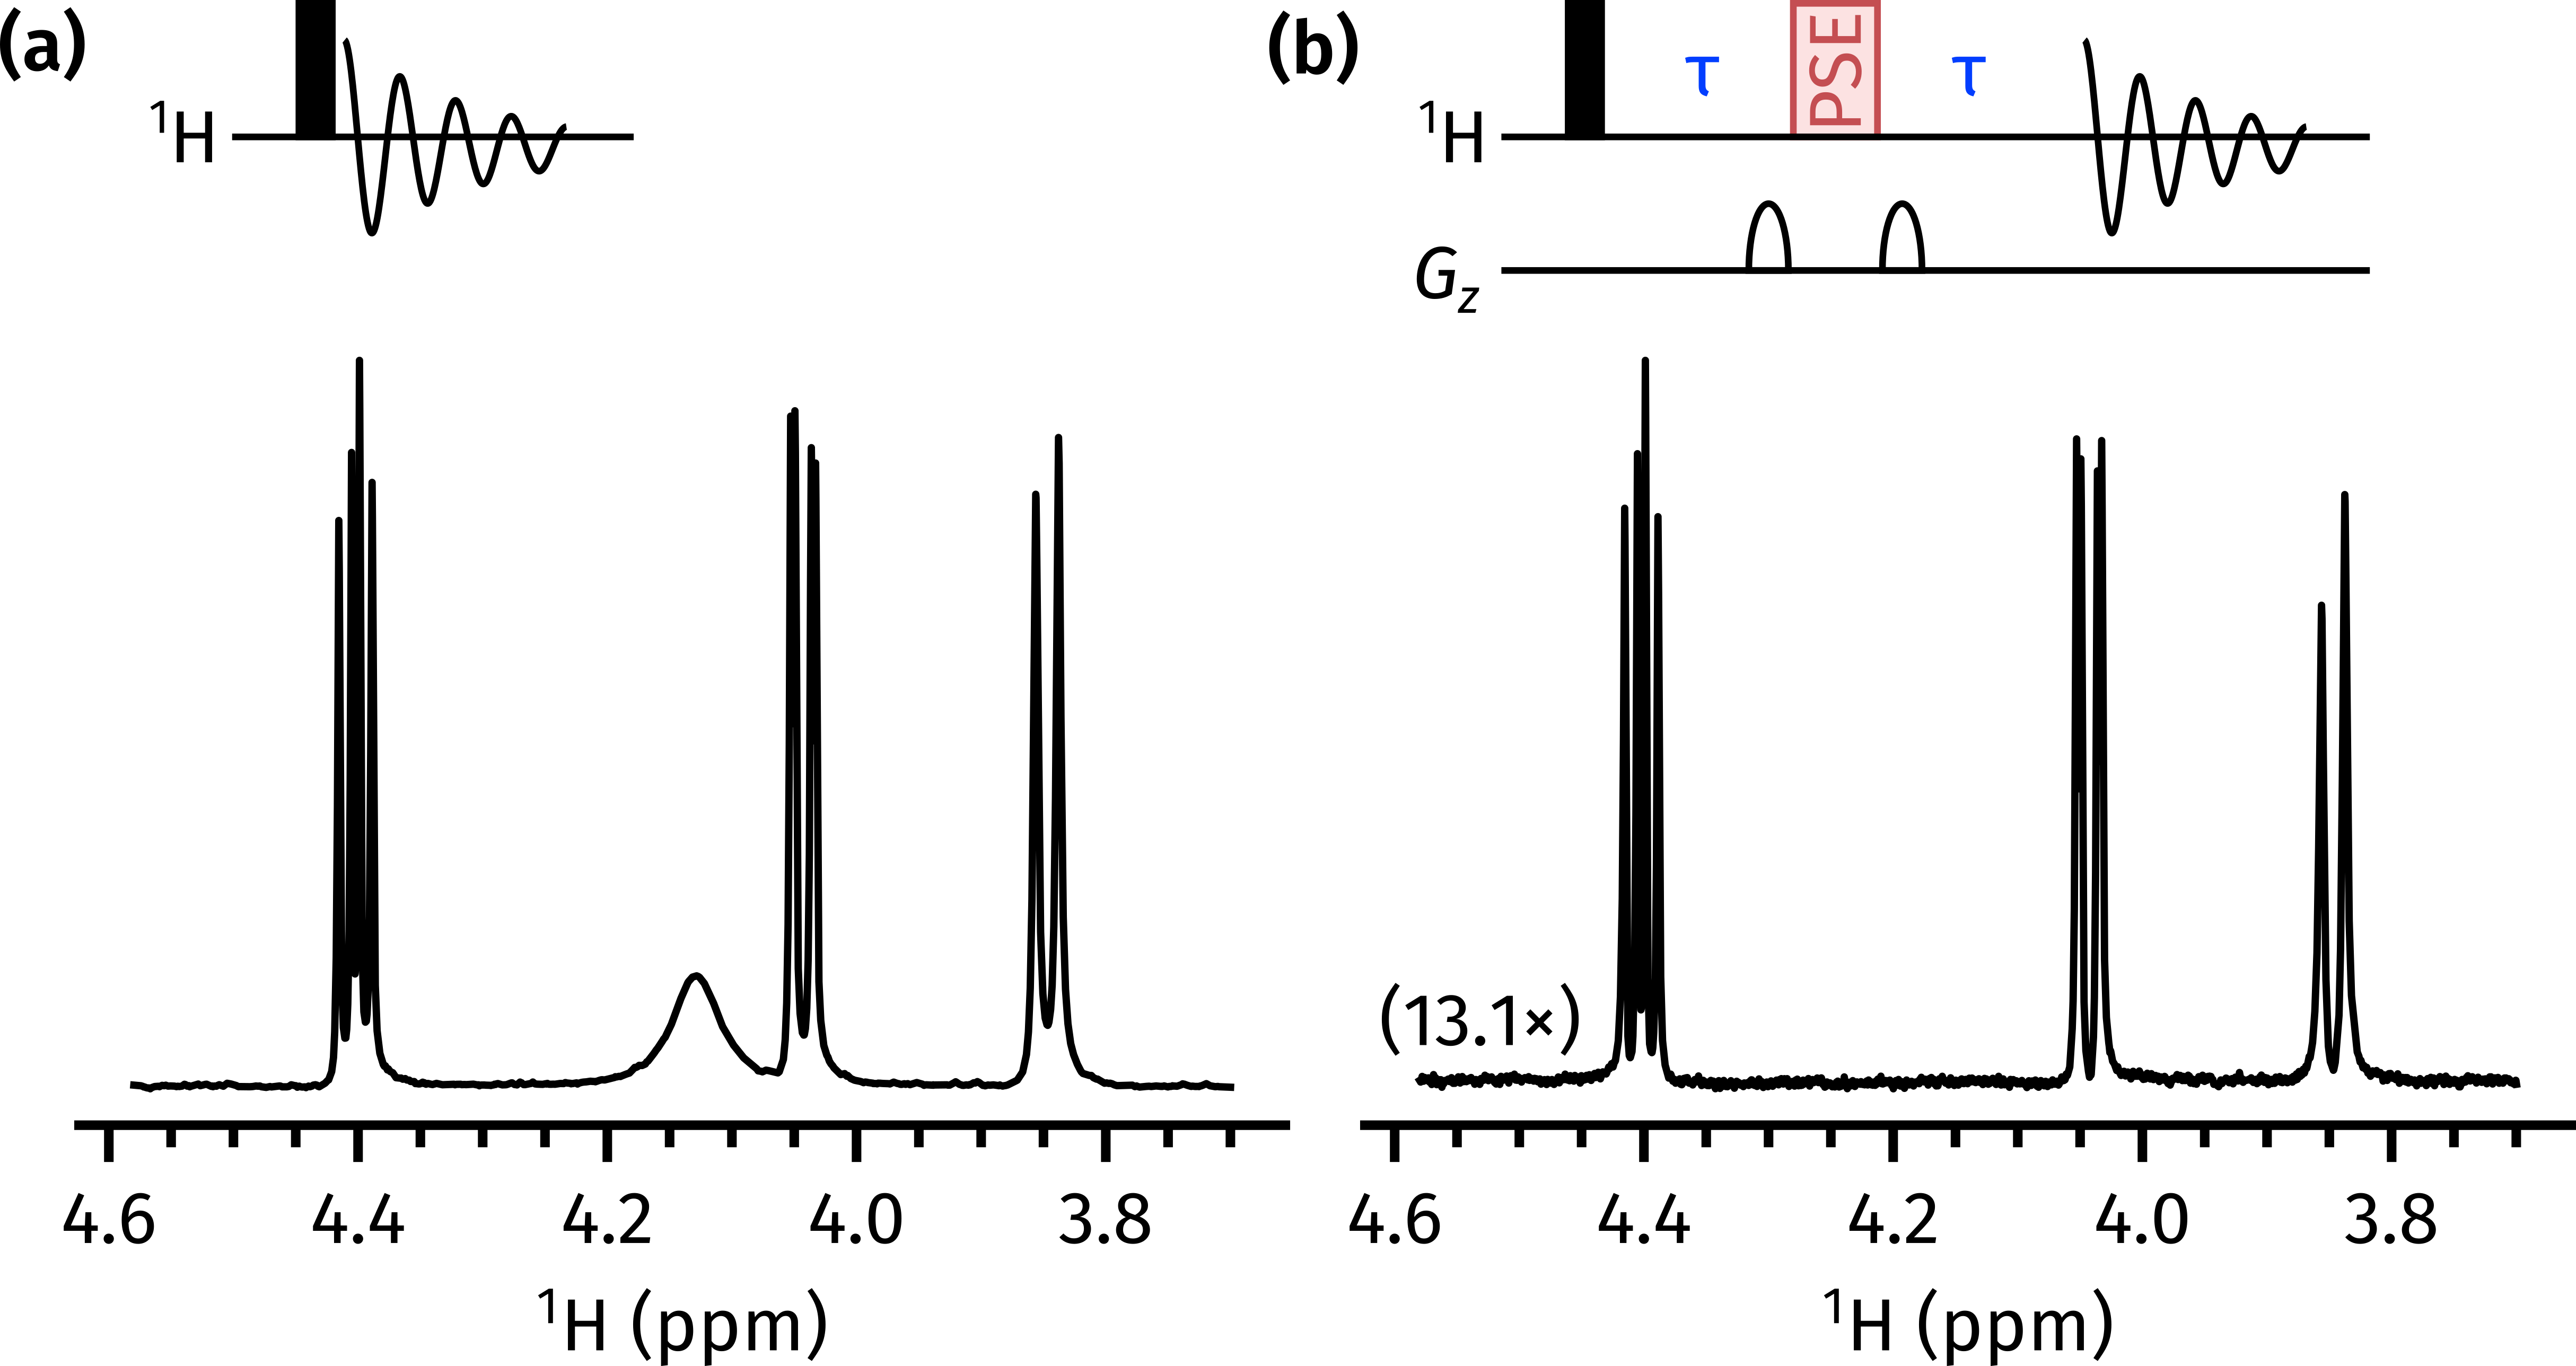
\includegraphics[]{pureshift/jrse.png}%
    {\phantomsubcaption\label{fig:jrse_zg}}%
    {\phantomsubcaption\label{fig:jrse_jrse}}%
    \caption[J-refocused spin echo experiment]{
        \textbf{(\subref*{fig:jrse_zg})} Pulse--acquire experiment and the resulting spectrum.
        \textbf{(\subref*{fig:jrse_jrse})} J-refocused spin echo experiment and the resulting spectrum.
        The PSE used was the PSYCHE double saltire, with a flip angle of \ang{25}; the delay $\tau$ was \qty{11}{\ms}.
        The OH peak at \qty{4.1}{ppm} is lost, most likely due to chemical exchange.
        \datacode{6A-200816}
    }
    \label{fig:jrse}
\end{figure}

Two cost functions were designed and used in this section:
\begin{align}
    f_\text{phase} &= \Var_i\left[\arctan\left(\frac{S_{\text{re},i}}{|S_{\text{im},i}|}\right)\right] \label{eq:ps_cf_phase} \\
    f_\text{diff} &= \Biggl\lVert \frac{\symbf{S}_\text{re}}{\lVert \symbf{S}_\text{re} \rVert} - \frac{\symbf{T}_\text{re}}{\lVert \symbf{T}_\text{re} \rVert} \Biggr\rVert, \label{eq:ps_cf_diff}
\end{align}
where the JRSE and pulse--acquire 1D spectra are treated as complex-valued vectors $\symbf{S}$ and $\symbf{T}$ respectively (for \textit{`spectrum'} and \textit{`target'}). $\symbf{S}_\text{re}$ and $\symbf{S}_\text{im}$ are the real and imaginary parts of the spectrum $\symbf{S}$, and $S_{\text{re},i}$ is the $i$-th point of the real part of the spectrum.
The operator $\Var_i$ represents the variance over all points in the spectrum (indexed by $i$), and $\lVert \symbf{x} \rVert$ denotes the 2-norm of the vector $\symbf{x}$, i.e.\ $\sqrt{\sum_i x_i^2}$.
Python implementations of these are given in \cref{lst:pureshift_costfunctions}.%
\footnote{The use of \texttt{np.arctan} (the arctangent), and \textit{not} \texttt{np.arctan2} (the argument of a complex number), is intentional. The behaviour shown in \cref{fig:fa_scan_synthetic} isn't reproduced with \texttt{arctan2}. Of course, this means the name `phase' is a misnomer; it's not really the phase of anything meaningful.}

\begin{mylisting}[htb]
\begin{tcbminted}{python}
import numpy as np
# assume S and T are complex numpy arrays which have been read in
Sr = np.real(S); Si = np.imag(S); Tr = np.real(T)
f_phase = np.var(np.arctan(Sr / np.abs(Si)))
f_diff = np.linalg.norm((Sr / np.linalg.norm(Sr))
                        - (Tr / np.linalg.norm(Tr)))
\end{tcbminted}
    \caption[Pure shift cost functions]{Pure shift cost functions.}
    \label{lst:pureshift_costfunctions}
\end{mylisting}

\begin{figure}[htb]
    \centering
    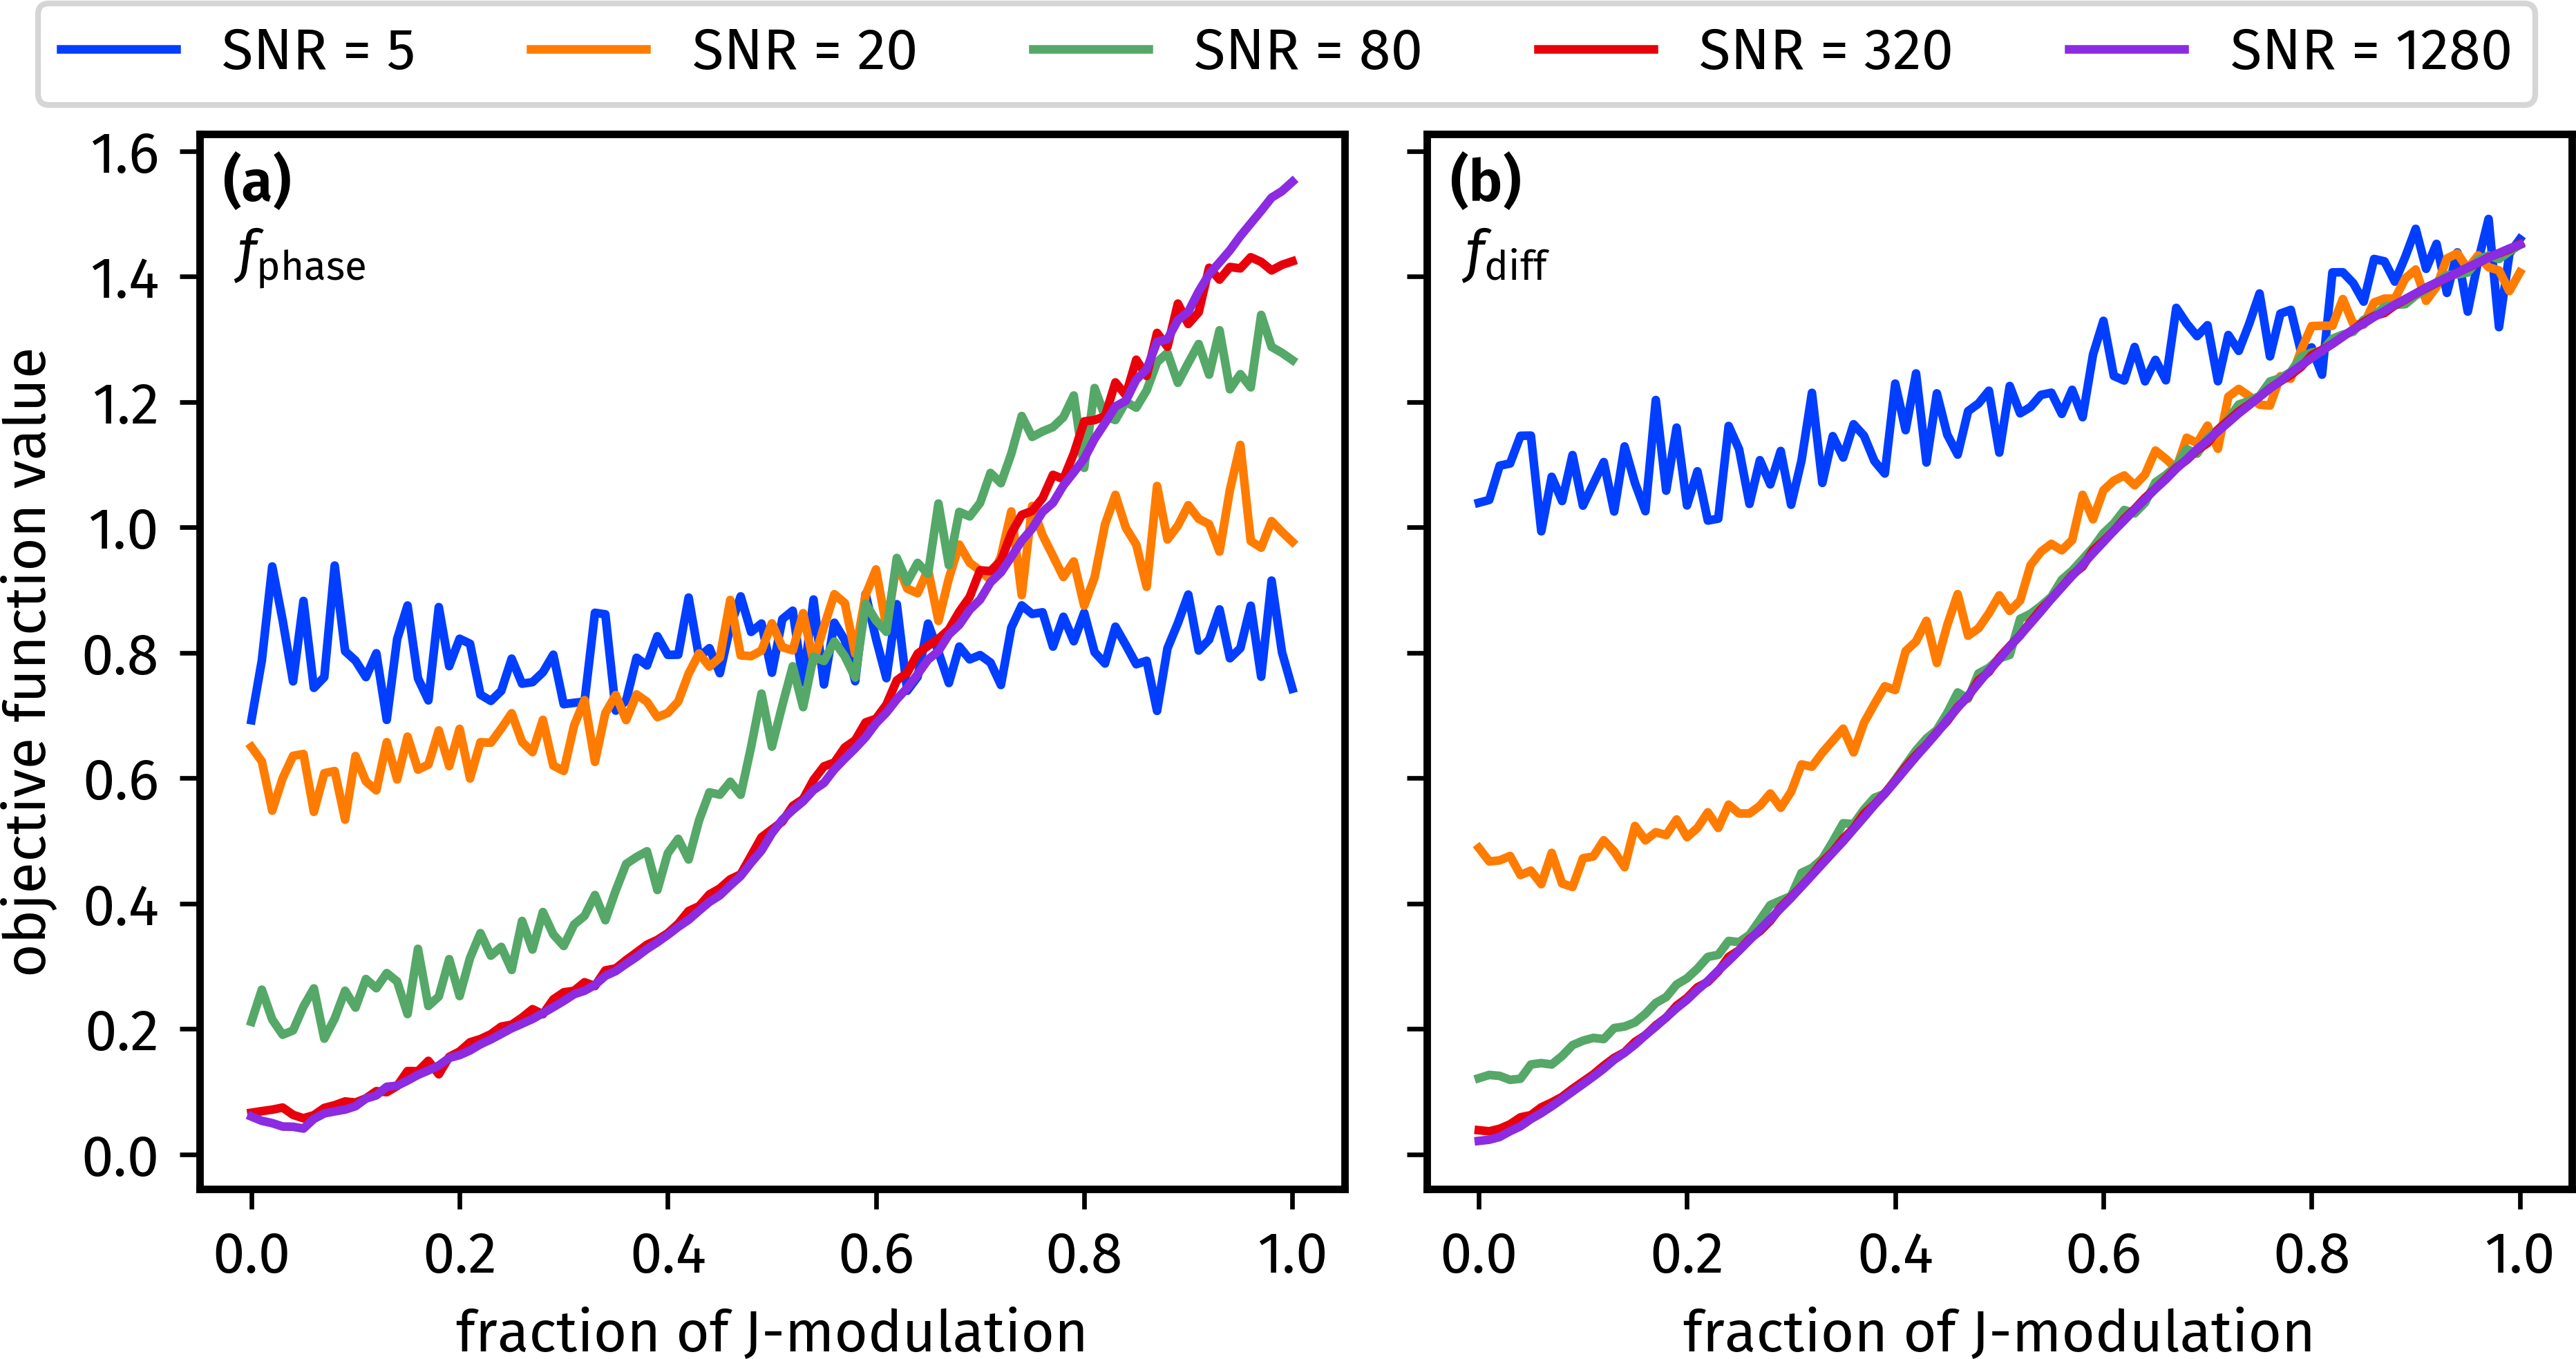
\includegraphics[]{pureshift/fa_scan_synthetic.png}%
    {\phantomsubcaption\label{fig:fa_scan_synthetic_fphase}}%
    {\phantomsubcaption\label{fig:fa_scan_synthetic_fdiff}}%
    \caption[Evaluation of $f_\text{phase}$ and $f_\text{diff}$ cost functions on synthetic data]{
        Behaviour of the two cost functions, $f_\text{phase}$ and $f_\text{diff}$, on synthetic spectra with various SNRs.
        Zero phase distortion refers to an in-phase absorption-mode doublet, whereas complete phase distortion refers to an antiphase dispersion-mode doublet.
        \textbf{(\subref*{fig:fa_scan_synthetic_fphase})} The $f_\text{phase}$ cost function.
        \textbf{(\subref*{fig:fa_scan_synthetic_fdiff})} The $f_\text{diff}$ cost function, measured against a spectrum with no phase distortion and an SNR of 500.
    }
    \label{fig:fa_scan_synthetic}
\end{figure}

These two cost functions were chosen as they exhibited desirable characteristics on synthetic data (\cref{fig:fa_scan_synthetic}).
In these simulations, the `target' spectrum was chosen to simply be an in-phase absorption-mode doublet with an SNR of 500.
Synthetic data with increasing amounts of J-modulation (i.e.\ spectra ranging from in-phase absorption, to antiphase dispersion) were generated, and extra Gaussian noise added to mimic different SNRs.
It can be seen that, for data which have little J-modulation (left edges of the plots), both $f_\text{phase}$ (\cref{fig:fa_scan_synthetic_fphase}) and $f_\text{diff}$ (\cref{fig:fa_scan_synthetic_fdiff}) penalise lower SNRs.
Furthermore, both of the cost functions penalise J-modulation, since they increase going from left to right.
This penalty is stricter for high-SNR spectra, which is also desirable, since it is only in high-SNR spectra that the J-modulation becomes noticeable.

The cost function $f_\text{diff}$ is easier to comprehend: it simply scales both the target and JRSE spectra down by their respective intensities, and compares each point to determine whether the peak shapes obtained are similar.
Although this seems like it should be agnostic towards signal intensity, this is only true for noiseless spectra.
If a (genuine) JRSE spectrum has low SNR, $\lVert \symbf{S}_\text{re} \rVert$ will be small, and the noise will be scaled down less than for the target spectrum; this difference in the \textit{noise} (rather than the signal) then contributes towards the cost function.
On the other hand, a proper rationalisation of why the cost function $f_\text{phase}$ works is unfortunately not within my capabilities!
It was mostly developed by trial-and-error (based on the notion that phase distortions would have something to do with $\symbf{S}_\text{re}$ and $\symbf{S}_\text{im}$), and I do not have a good explanation of why it works.

\begin{figure}[htbp]
    \centering
    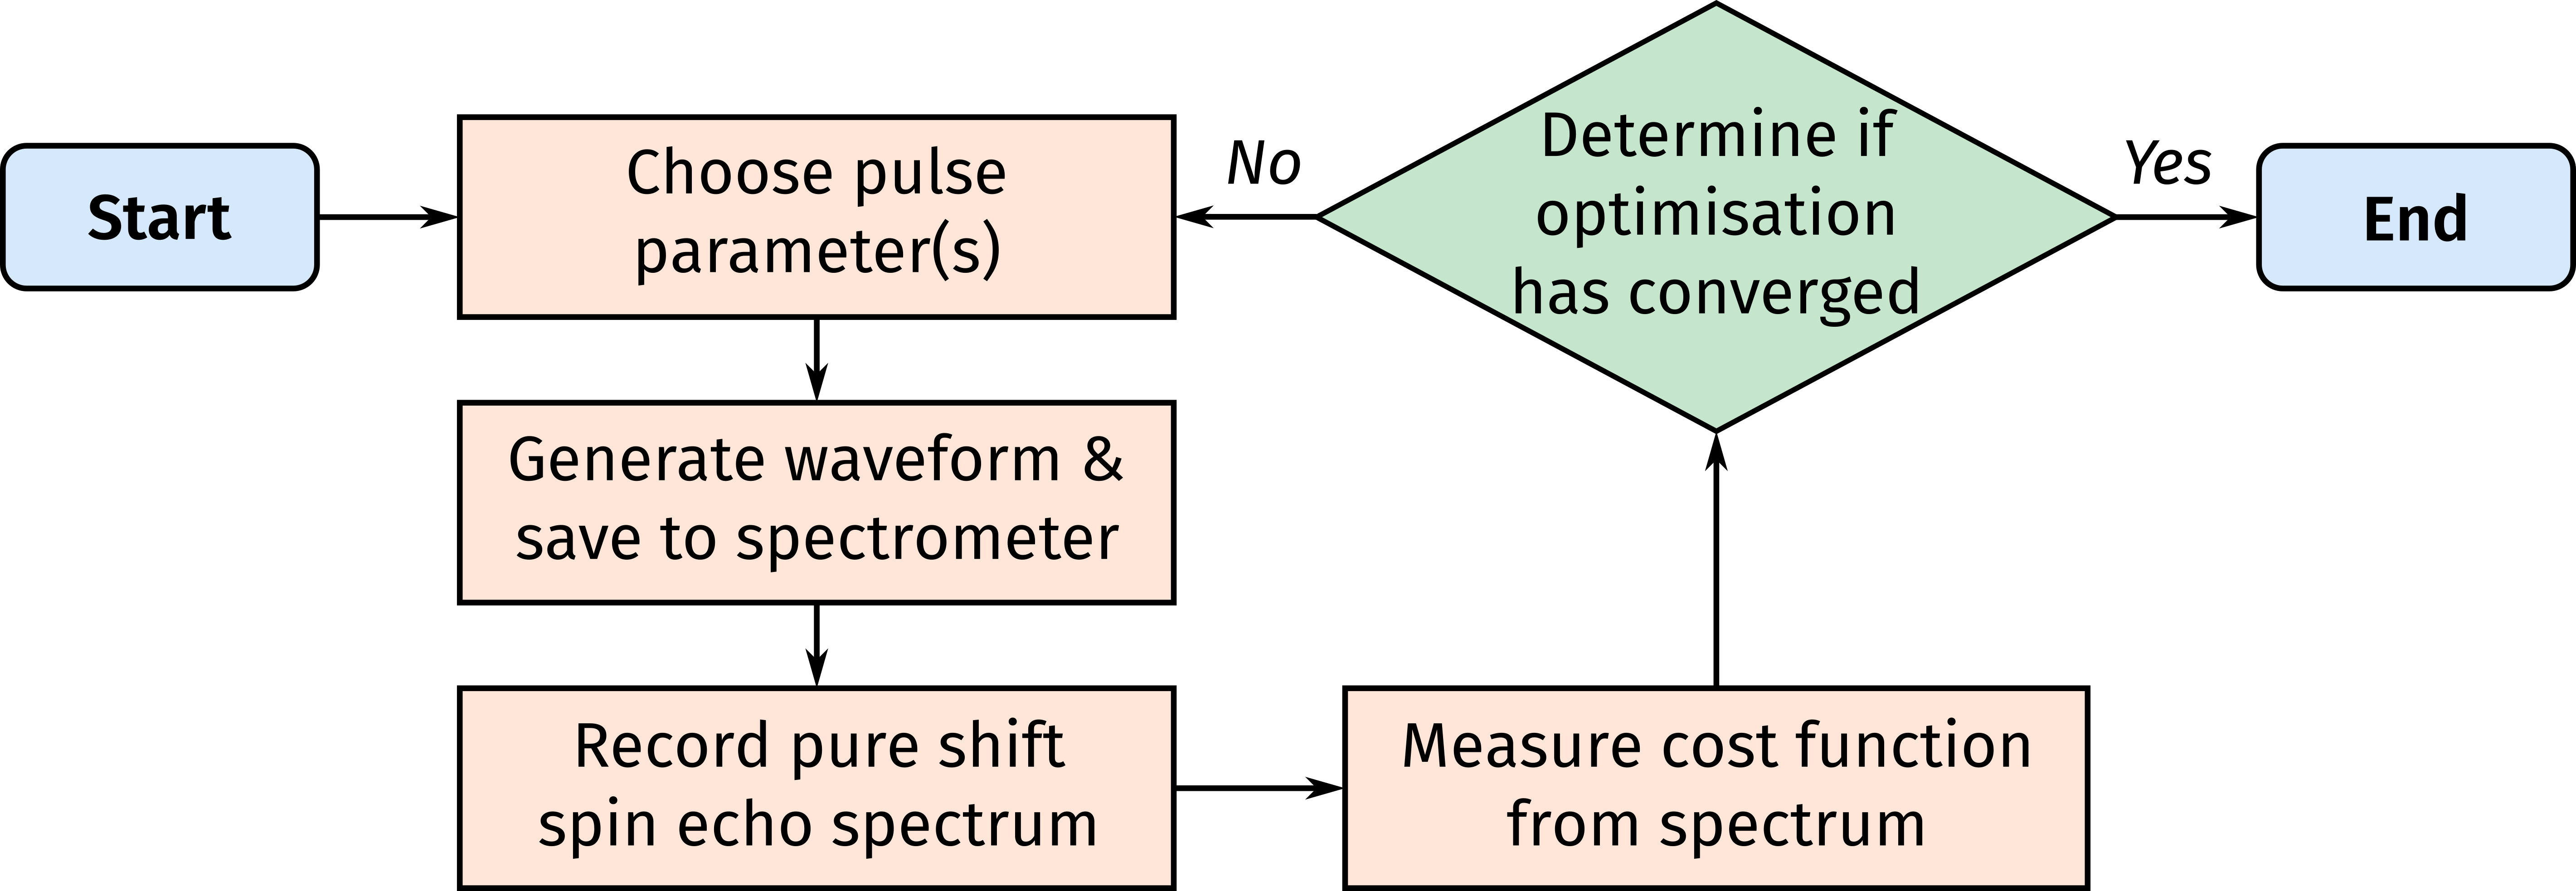
\includegraphics[]{pureshift/optim_flowchart_early.png}%
    \caption[Flowchart for pure shift optimisation process]{
        Flowchart illustrating the steps for optimisation of a pure shift spectrum.
    }
    \label{fig:optim_flowchart_early}
\end{figure}

The general optimisation procedure is conceptually simple and largely consists of the loop shown in \cref{fig:optim_flowchart_early}: this is essentially a specialised version of the POISE flowchart (\cref{fig:poise_flowchart}).
The optimisation algorithm is responsible for determining convergence, as well as choosing the new parameters based on previously obtained information; the initial parameters must be supplied by the user.

In practice, it is a technical challenge to implement this loop on a spectrometer as the cost function calculation is performed either in Matlab or Python 3, both of which are not compatible with Bruker's TopSpin software.
TopSpin instead provides Jython (Python 2.7) and C programming interfaces;%
\footnote{TopSpin 4.1.4 introduced a Python 3 interface which would have made much of this work simpler. Unfortunately, this was not available at the time of this work.}
the former is not compatible with Python 3 packages like \texttt{numpy} or \texttt{scipy}, and the latter is too low-level to be worth implementing numerical algorithms in.%
\footnote{Of course, heavily optimised code in low-level languages such as C and Fortran---or perhaps even Matlab---would run faster. However, speeding up the code has virtually no impact on the optimisation, since its rate is limited by spectrum acquisition. In this situation, it makes far more sense to save \textit{developer time}.}
Thus, we require a means of \textit{communication} between the spectrometer and the optimisation control programme: this includes a signal from the controlling programme to trigger acquisition on the spectrometer, as well as a signal from the spectrometer that acquisition is done so that the cost function can be calculated.
As it turns out, the code used for the optimisations in this section was a very rudimentary and fragile form of that eventually used in POISE (for example, the aforementioned signals were transmitted via the creation and deletion of files).
I therefore defer the discussion of this issue to \cref{subsec:poise__implementation}, where the more robust POISE interface is explained in detail.
